\subsection{Manuscript Management}
\subsubsection{Creating a Manuscript}
\textbf{Using the Wizard}\\
	Creating a manuscript (e.g. book, letter, poem, etc.), is a very easy process. The manuscript you've created will be available to you immediately after creation. At which point you may edit it as you wish. Let us have a look at the steps necessary to creating your masterpiece.\\ \\

	\begin{itemize}
		\item Assuming that logging in has been successfully achieved, the location should be the homepage of Figbook. Click on "Catalogue" on the top-leftmost block on the blocks on the screen. You should now see this page:
		
		\begin{figure}[h]
		\centering
			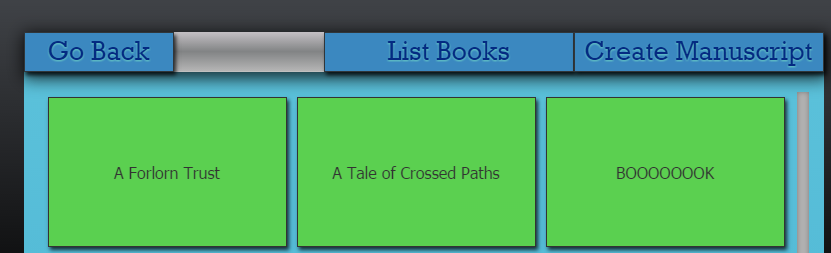
\includegraphics[scale=0.5]{images/viewBooks.png}
			\caption{Create Manuscript button}
		\end{figure}
		
		Click 'Create Manuscript' to open the wizard.
		\item The book title, author name and author surname should be entered. Click next when done, or back to return to the previous page.
		
		\begin{figure}[h]
			\centering
			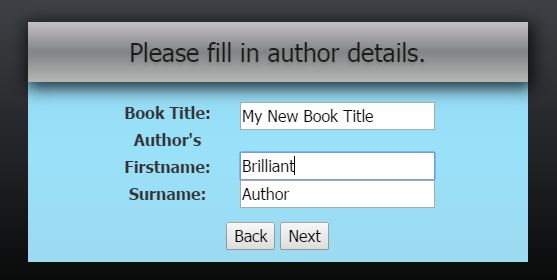
\includegraphics[scale=0.5]{images/createManuscriptWizard.png}
			\caption{Entering details of the book}
		\end{figure}
		\item A preface on the content of the book should be entered. It clear and decriptive to optimize the quality of the selected piece of literature (Note that this is not compulsory. You may leave it blank). 
		
		\begin{figure}[h]
		\centering
			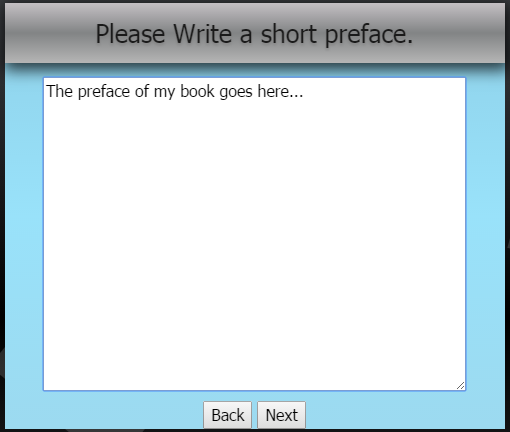
\includegraphics[scale=0.5]{images/preface.png}
			\caption{Entering preface of the book}
		\end{figure}
	
		\item Clicking next will create your manuscript and return you to your list of books. Your manuscript will be listed there. You can click on it to start editing.
		\end{itemize}
\subsubsection{Editing a Manuscript}
	Editing a manuscript entails loading the content of an existing manuscript into an open text area for the author to edit. 

	\begin{itemize}
		\item To access all the manuscripts available to you, from the home page click on the 'Catalogue' button. This should populate the page with all the manuscripts available to the user. 
		\begin{figure}[h]
			\centering
			
\includegraphics[scale=0.5]{images/catalogue.png}
			\caption{catalogue button on home page}
		\end{figure} 
		
		\newpage
		\item Open a manuscript by clicking on it. This should take you to the document layout of the manuscript of interest. Click on 'edit' next to any section to open the text area.
		\begin{figure}[h]
			\centering
			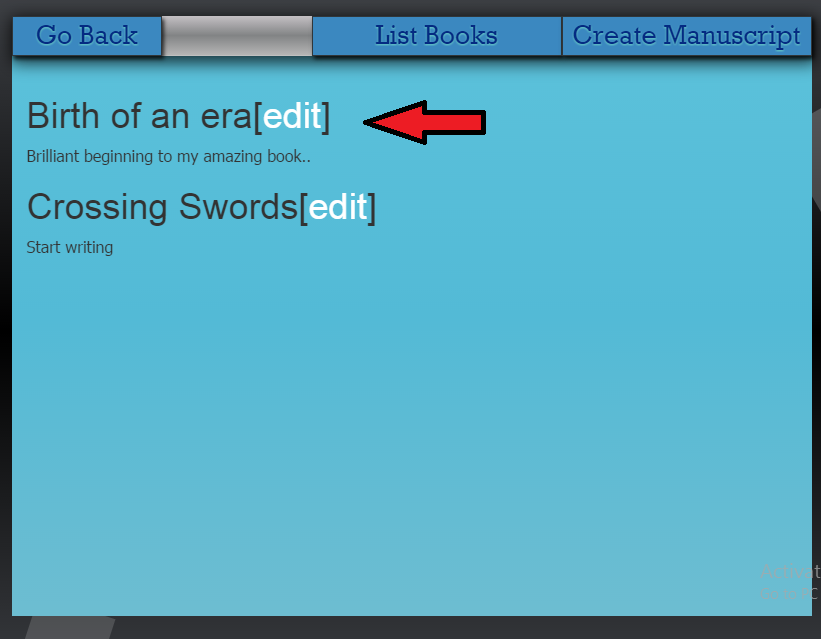
\includegraphics[scale=0.5]{images/editLink.png}
			\caption{links to edit a section of the manuscript}
		\end{figure} 
		\item you may edit any area of the section and click the 'Save' button when you wish to save the changes made. This should take you back to the document view of the manuscript.
		
		\begin{figure}[h]
			\centering
			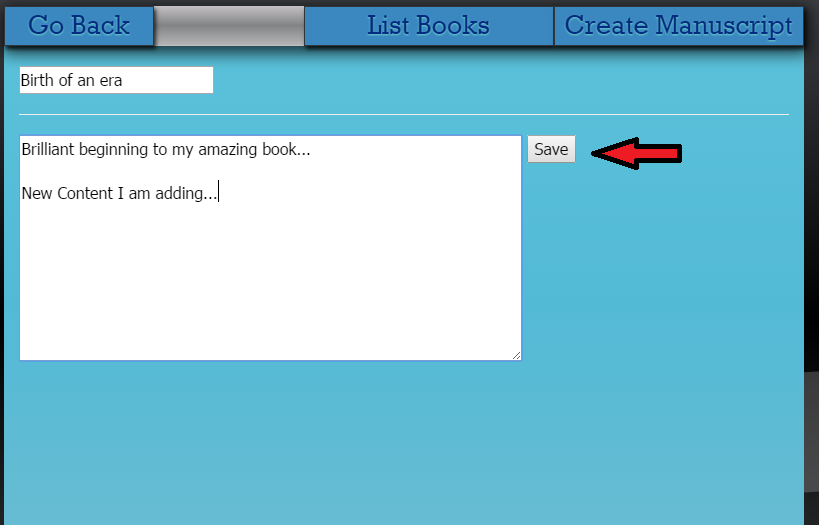
\includegraphics[scale=0.5]{images/saveManuscriptSection.png}
			\caption{save section button}
		\end{figure} 
		
		\item Assuming that logging in has been successfully achieved, the location should be the homepage of Figbook. A button 'Create Manuscript' should be available. Click on the button to open the wizard.
		\item The book title, author name and author surname should be entered. Click next when done. 
		\item A preface on the content of the book should be entered. It clear and decriptive to optimize the quality of the selected piece of literature.
		\item Some text needs to be added to the textbox that appears after the preface of the book has been added.
	\end{itemize}

\subsection{Editing a Manuscript}
	Editing a manuscript entails loading the content of an existing manuscript into an open text area for the author to edit. Only a single author is allowed to edit a single section at a time and failure to do so will result in a editing conflict. 

	\begin{itemize}
		\item To access all the manuscripts available to you, click on the 'List Manuscripts' button. This should populate the page with all the manuscripts available to the user. 
		\item Open a manuscript by clicking on it. This should take you to the document layout of the manuscript of interest. Click on any section to open the text area. Be vigilent in communicating with any collaborators because if two or more authors edit the same section at the same time, this will result in merging conflicts when trying to save.
		\item you may edit any area of the section and click the 'Save' button when you wish to save the changes made. This should take you back to the document view of the manuscript.
	\end{itemize}